\documentclass[twoside]{article}

%
% This is a borrowed LaTeX template file for lecture notes for CS267,
% Applications of Parallel Computing, UCBerkeley EECS Department.
% Now being used for CMU's 10725 Fall 2012 Optimization course
% taught by Geoff Gordon and Ryan Tibshirani.  When preparing 
% LaTeX notes for this class, please use this template.
%
% To familiarize yourself with this template, the body contains
% some examples of its use.  Look them over.  Then you can
% run LaTeX on this file.  After you have LaTeXed this file then
% you can look over the result either by printing it out with
% dvips or using xdvi. "pdflatex template.tex" should also work.
%

\setlength{\oddsidemargin}{0.25 in}
\setlength{\evensidemargin}{-0.25 in}
\setlength{\topmargin}{-0.6 in}
\setlength{\textwidth}{6.5 in}
\setlength{\textheight}{8.5 in}
\setlength{\headsep}{0.75 in}
\setlength{\parindent}{0 in}
\setlength{\parskip}{0.1 in}

%
% ADD PACKAGES here:
%

\usepackage{amsmath,amsfonts,graphicx}

%
% The following commands set up the lecnum (lecture number)
% counter and make various numbering schemes work relative
% to the lecture number.
%
\newcounter{lecnum}
\renewcommand{\thepage}{\thelecnum-\arabic{page}}
\renewcommand{\thesection}{\thelecnum.\arabic{section}}
\renewcommand{\theequation}{\thelecnum.\arabic{equation}}
\renewcommand{\thefigure}{\thelecnum.\arabic{figure}}
\renewcommand{\thetable}{\thelecnum.\arabic{table}}

%
% The following macro is used to generate the header.
%
\newcommand{\lecture}[4]{
   \pagestyle{myheadings}
   \thispagestyle{plain}
   \newpage
   \setcounter{lecnum}{#1}
   \setcounter{page}{1}
   \noindent
   \begin{center}
   \framebox{
      \vbox{\vspace{2mm}
    \hbox to 6.28in { {\bf Econ 626: Quantitative Methods II
  \hfill Fall 2018} }
       \vspace{4mm}
       \hbox to 6.28in { {\Large \hfill Lecture #1: #2  \hfill} }
       \vspace{2mm}
       \hbox to 6.28in { {\it Lecturer: #3 \hfill Scribes: #4} }
      \vspace{2mm}}
   }
   \end{center}
   \markboth{Lecture #1: #2}{Lecture #1: #2}

   %{\bf Note}: {\it LaTeX template courtesy of UC Berkeley EECS dept.}

   {\bf Disclaimer}: {\it Zhikun is fully responsible for the errors and typos appeared in the notes.}
   \vspace*{4mm}
}
%
% Convention for citations is authors' initials followed by the year.
% For example, to cite a paper by Leighton and Maggs you would type
% \cite{LM89}, and to cite a paper by Strassen you would type \cite{S69}.
% (To avoid bibliography problems, for now we redefine the \cite command.)
% Also commands that create a suitable format for the reference list.
\renewcommand{\cite}[1]{[#1]}
\def\beginrefs{\begin{list}%
        {[\arabic{equation}]}{\usecounter{equation}
         \setlength{\leftmargin}{2.0truecm}\setlength{\labelsep}{0.4truecm}%
         \setlength{\labelwidth}{1.6truecm}}}
\def\endrefs{\end{list}}
\def\bibentry#1{\item[\hbox{[#1]}]}

%Use this command for a figure; it puts a figure in wherever you want it.
%usage: \fig{NUMBER}{SPACE-IN-INCHES}{CAPTION}
\newcommand{\fig}[3]{
      \vspace{#2}
      \begin{center}
      Figure \thelecnum.#1:~#3
      \end{center}
  }
% Use these for theorems, lemmas, proofs, etc.
\newtheorem{theorem}{Theorem}[lecnum]
\newtheorem{lemma}[theorem]{Lemma}
\newtheorem{proposition}[theorem]{Proposition}
\newtheorem{claim}[theorem]{Claim}
\newtheorem{corollary}[theorem]{Corollary}
\newtheorem{definition}[theorem]{Definition}
%\newtheorem{example}[theorem]{Example}
\newenvironment{proof}{{\bf Proof:}}{\hfill\rule{2mm}{2mm}}
\newenvironment{example}{{\bf Example:}}{\hfill\rule{2mm}{2mm}}

\newtheorem{remark}[theorem]{Remark}
%\newenvironment{remark}[1][Remark]{\begin{trivlist}\item[\hskip \labelsep {\bfseries #1}]}{\end{trivlist}}


% **** IF YOU WANT TO DEFINE ADDITIONAL MACROS FOR YOURSELF, PUT THEM HERE:

\newcommand\E{\mathbb{E}}
\newcommand\dd{\mathrm{d}}

\usepackage{hyperref}
\usepackage{cancel}
\usepackage{listings}
\newcommand\pp{\partial}
\newcommand\pd{\partial}
\newcommand\imp{$\Longrightarrow$}
\newcommand\lb{\left (}
\newcommand\rb{\right )}
\newcommand\lsb{\left [}
\newcommand\rsb{\right ]}
\newcommand\lcb{\left \{}
\newcommand\rcb{\right \}}

\begin{document}
%FILL IN THE RIGHT INFO.
%\lecture{**LECTURE-NUMBER**}{**DATE**}{**LECTURER**}{**SCRIBE**}
\lecture{7}{Back to Dynamic Programming}{Prof. Daniel Levy}{Zhikun Lu}
%\footnotetext{These notes are partially based on those of Nigel Mansell.}
\footnotetext[1]{Visit \url{http://www.luzk.net/misc} for updates.}

\hfill Date: September 6, 2018

\section{Stochastic Model}
\begin{equation}
    \max\limits_{\lcb C_t, K_{t+1} \rcb} \quad \E_{0} \lsb \sum_{t=0}^{\infty} \beta^{t} u(C_{t})  \rsb 
\end{equation}
\begin{equation}
    \text{s.t.} \quad C_t + K_{t+1} = Z_{t}f(K_{t})
\end{equation}
where $\E_{0} = E \{ \cdot | \Omega_{0} \}$. Optimal choices here are contingency plans.

$\{ K_{t}, Z_{t} \}$ are state variables. $K_{t+1}$ and $C_{t}$ will be a function of $K_{t}$ and $Z_{t}$. Since $Z$ is a r.v., $K_{t+1}$ and $C_t$ will also be r.v.'s.

\underline{Bellman's Equation}
\begin{equation}
    V(K_{t}, Z_{t}) = \begin{cases}
        \max ~ [u(C_{t}) + \beta \E_t V(K_{t+1}, Z_{t+1})]\\
        \text{s.t.} \quad C_{t} + K_{t+1} = Z_{t} f(K_{t})
    \end{cases}
\end{equation}
i.e.
\begin{equation}
    V(K_{t}, Z_{t}) = \begin{cases}
        \max ~ [u(C_{t}) + \beta \int V(K_{t+1}, Z_{t+1}) h(Z_{t+1}) \dd Z_{t+1}]\\
        \text{s.t.} \quad C_{t} + K_{t+1} = Z_{t} f(K_{t})
    \end{cases}
\end{equation}
where $h(\cdot)$ is the conditional p.d.f. of $Z_{t+1}$, given that the p.d.f. conditonal on $\Omega_{t}$ exists.

\underline{Lagrangian}
\begin{equation}
    V(K_{t}, Z_{t}) = u(C_{t}) + \beta \E_t V(K_{t+1}, Z_{t+1}) + \lambda_{t} [Z_{t} f(K_{t}) - C_{t} - K_{t+1}]
\end{equation}

\underline{FONC}
\begin{equation}
    \E_{t}[u'(C_{t}) - \lambda_{t}] = 0 \Longrightarrow \lambda_{t} = u'(C_{t})
\end{equation}
\begin{equation}
    \E_{t}[\beta V'_{K_{t+1}}(K_{t+1}, Z_{t+1}) - \lambda_{t} ] = 0 \Longrightarrow \lambda_{t} = \beta \E_{t} V'_{K_{t+1}}(K_{t+1}, Z_{t+1})
\end{equation}
\imp
\begin{equation}
    u'(C_{t}) = \beta \E_t V'_{K_{t+1}}(K_{t+1}, Z_{t+1})
\end{equation}

\underline{Note:}
\begin{equation}
    \Omega_{t} = \lcb K_{t-j}, C_{t-j}, Z_{t-j} | j = 0,1,...  \rcb
\end{equation}
Based on the B-S Theorem, we can write
\begin{equation}
    V'_{K_{t}}(K_{t}, Z_{t}) = \lambda_{t} Z_{t} f'(K_{t}) = u'(C_{t} )Z_{t} f'(K_{t})
\end{equation}
Lead (7.10) \imp
\begin{equation}
    u'(C_{t}) = \beta \E_{t} u'(C_{t+1} )Z_{t+1} f'(K_{t+1})
\end{equation}

\underline{Assumption}
\begin{eqnarray}
    f(K_{t}) &=& K_{t}^{\alpha}\\
    u(C_{t}) &=& \ln C_{t}
\end{eqnarray}
\imp
\begin{equation}
    \frac{1}{C_{t}} = \beta \E_{t} \frac{1}{C_{t+1}} Z_{t+1} \alpha (K_{t+1})^{\alpha - 1}
\end{equation}
Guess
\begin{eqnarray}
    K_{t+1} &=& \theta Z_{t} K_{t}^{\alpha}\\
    C_{t}   &=& (1- \theta)Z_{t}K_{t}^{\alpha}
\end{eqnarray}
(7.14) and (7.16) \imp
\begin{eqnarray}
    \frac{1}{(1- \theta)Z_{t}K_{t}^{\alpha}} &=& \beta \E_{t} \frac{1}{(1- \theta)\cancel{Z_{t+1}}K_{t+1}^{\alpha}} \cancel{Z_{t+1}} \alpha (K_{t+1})^{\alpha - 1}\\
    \frac{1}{(1- \theta)Z_{t}K_{t}^{\alpha}} &=& \alpha \beta \E_{t} \frac{1}{(1- \theta) K_{t+1}}\\
    \frac{1}{\cancel{(1- \theta)Z_{t}K_{t}^{\alpha}}} &=& \alpha \beta \E_{t} \frac{1}{\cancel{(1- \theta)} \theta \cancel{ Z_{t} K_{t}^{\alpha}}}\\
    1 &=& \alpha \beta \frac{1}{\theta}\\
    \Longrightarrow \quad \theta   &=& \alpha \beta
\end{eqnarray}
\imp
\begin{eqnarray}
    K^{*}_{t+1} &=& \alpha \beta Z_{t} K_{t}^{\alpha}\\
    C^{*}_{t}   &=& (1- \alpha \beta)Z_{t}K_{t}^{\alpha}
\end{eqnarray}

To say something about the properties of $K^{*}_{t+1}$ and $C^{*}_{t}$, we need to know the properties of $Z_{t}$.

\begin{example}
    \begin{equation}
        \ln Z_{t} \sim N(\mu, \sigma^{2}) \Longrightarrow Z_{t} \sim LN
    \end{equation}
    \underline{Recall} The MGF of $x \sim N(\mu, \sigma^{2})$ is given by 
    \begin{equation}
        M_{x}(t) = e^{\mu t + \frac{\sigma^{2}t^{2}}{2}} 
    \end{equation} 
    Since $\ln Z_{t} \sim N(\mu, \sigma^{2})$, PDF of $\ln Z_{t}$ is given by \begin{equation}
        f(\ln Z_{t}) = \frac{1}{Z_{t} \sigma \sqrt{2\pi}}e^{-\frac{(\ln Z_{t} - \mu)^{2}}{2 \sigma^{2}}}
    \end{equation}
    \underline{Recall} 
    \begin{equation}
        M_{y}(t) = \E \left[ e^{t y} \right] = \E \left[ e^{t \ln Z} \right] = \E \left[ Z^{t} \right] 
    \end{equation}
    \begin{equation}
        M_{\ln Z}(t) = \E \left[ Z^{t} \right] 
    \end{equation}
    \begin{equation}
        \E \left[ Z \right] = M_{\ln Z}(1) = e^{\mu + \frac{\sigma^{2}}{2}}
    \end{equation}
    \begin{equation}
         Var(Z) = \E \left[ Z^{2} \right] - (\E \left[ Z \right])^{2} =  M_{\ln Z}(2) -  (M_{\ln Z}(1))^{2} = e^{2 \mu + 2 \sigma^{2}} - (e^{\mu + \frac{\sigma^{2}}{2}})^{2} = e^{2 \mu + \sigma^{2}} ( e^{\sigma^{2}} - 1)
    \end{equation} 
    Since $Z_{t}$ is log-normal, so are $K^{*}_{t+1}$ and $C^{*}_{t}$.
    \begin{eqnarray}
        K_{t+1} &=& \alpha \beta Z_{t} K^{\alpha}_{t}\\
        \ln K_{t+1} &=& \ln \alpha \beta + \ln Z_{t} + \alpha \ln K_{t}\\
        \ln K_{t} &=& \ln \alpha \beta + \ln Z_{t-1} + \alpha \ln K_{t-1}\\
        \ln K_{t-1} &=& \ln \alpha \beta + \ln Z_{t-2} + \alpha \ln K_{t-2}\\
        \ln K_{t} &=& \ln \alpha \beta + \ln Z_{t-1} + \alpha (\ln \alpha \beta + \ln Z_{t-2} + \alpha \ln K_{t-2})\\
        &=& (1+\alpha) \ln \alpha \beta + \ln Z_{t-1} + \alpha \ln Z_{t-2} + \alpha^{2} \ln K_{t-2}\\
        &=& (1+\alpha+ \alpha^{2}) \ln \alpha \beta + \ln Z_{t-1} + \alpha \ln Z_{t-2} + \alpha^{2} \ln Z_{t-3} + \alpha^{3} \ln K_{t-3}\\
        &\vdots& \notag\\
        &=& \ln \alpha \beta \sum_{i=0}^{t-1} \alpha^{i} + \sum_{i=0}^{t-1} \alpha^{i} \ln Z_{t-i-1} + \alpha^{t} \ln K_{0}
    \end{eqnarray}
    As $t \to \infty$, $\alpha^{t}\ln K_{0} \to 0$.
    \begin{equation}
        \lim_{t \to \infty} \E ( \ln K_{t}) = \frac{1}{1-  \alpha} \ln \alpha \beta + \sum_{i=0}^{\infty} \alpha^{i} \E \ln Z_{t-i-1} = \frac{1}{1-  \alpha} \ln \alpha \beta + \frac{1}{1 - \alpha} \mu
    \end{equation}
    \begin{equation}
        Var[\lim_{t \to \infty} \ln K_{t}] = \E [\lim_{t \to \infty} \ln K_{t}]^{2} - \lcb \E \left[ \lim_{t \to \infty} \ln K_{t} \right]  \rcb^{2}= ... = \frac{\sigma^{2}}{1 - \alpha^{2}}
    \end{equation}
\end{example}

\section{Funtionals}
\underline{Functionals}:
A function that maps from any set $X$ to $\mathbb{R}$, $f: X \to \mathbb{R}$ is called a functional.

\underline{Operations on Functionals}
\begin{equation}
    (f \pm g)(x) = f(x) \pm g(x)
\end{equation}
\begin{equation}
    (\alpha f )(x) = \alpha f(x)
\end{equation}

\underline{Lemma}: Let $X$ be a set and let $F(X)$ be the set of all functionals on $X$. Show that $F(X)$ is a linear space.

\begin{proof}
    $\forall f, g \in F(X)$ and $\forall \alpha \in \mathbb{R}$ we have
    $$
        (f + g)(x) = f(x) + g(x)
    $$
    $$
        (\alpha f)(x) = \alpha f(x)
    $$
    and therefore
    $$(f+g): X \to \mathbb{R} \quad \text{and} \quad \alpha f: X \to \mathbb{R}$$.
    \imp $F(X)$ is closed under addition and scalar multiplication.
\end{proof}

\underline{Note}: the ``zero'' element in $F(X)$ is the constant function $f(x) = 0 ~ \forall ~ x \in X$.

\underline{Definition} A functional $f \in F(X)$ is \underline{bounded} if $\exists k \in \mathbb{R}$ s.t. $|f(x)| \leq k ~ \forall x \in X$.

\underline{Definition} For any set $X$, the $B(X)$ denote the set of all bounded functionals on $X$.

\underline{Note}: $B(X) \subseteq F(X)$.

\underline{Continuity in Metric Space}

Let $(X,d_{1})$ and $(Y,d_{2})$ be metric spaces and let $f: X \to Y$. Then $f$ is \underline{continuous} at $x_{0} \in X$ if $\forall \epsilon >  0, \exists \delta(x_{0},\epsilon) > 0$ , s.t. 
$$d_{1}(x, x_{0})< \delta(x_{0},\epsilon) \Longrightarrow d_{2}[f(x_{0}),f(x)] < \epsilon.$$

\underline{Uniform Continuity}

A function $f : (X,d_1) \to (Y,d_2)$ is \underline{uniformly continuous} on a subset $A \subset X$ if $\forall x, y \in X$ and $\forall \epsilon > 0, \exists \delta(\epsilon) >0$, independent of $x$ and $y$, s.t. $$d_{1}(x,y) < \delta(\epsilon) \Longrightarrow d_{2}(f(x),f(y)) < \epsilon.$$

\underline{Lipschitz Continuity}

Let $X$ and $Y$ be normed vactor space. Then, a function $f: X \to  Y $ is Lipschitz continuous if $\exists \beta > 0$, s.t. $\forall x, x_{0} \in X$, 
\[
    || f(x) - f(x_0) || \leq \beta || x - x_{0}||
\]

\underline{Note}:
\begin{equation}
    \frac{||f(x)-f(x_0)||}{||x-x_0||} \leq \beta
\end{equation}

\underline{Lemma} (Preservation of Cauchy Property under Uniform Continuity)

Let $f : X \to Y$ be uniformly continuous. If $\{ x_{n}\}$ is Cauchy in $X$, then $\{ f(x_{n}) \}$ is Cauchy in $Y$.

\begin{proof}
    Let $\epsilon > 0$. By uniformly continuity, $\exists \delta > 0$ s.t. $d(f(x_{n}), f(x_{m})) < \epsilon, \forall x_{m}, x_{n} \in X$, s.t. $d(x_m,x_n) < \delta$. Suppose that $\{x_{n}\}$ is Cauchy in $X$ \imp $\exists N \in \mathbb{N}$ s.t. $ d(x_m,x_n) < \delta \forall m, n > N$. Then by uniform continuity of $f$,
    $d(f(x_m), f(x_n)) < \epsilon ~ \forall m, n > N \Longrightarrow$ $f(x_n)$ is Cauchy.
\end{proof}

\underline{Theorem}

A continuous function on a compact domain is uniformly continuous.

\underline{Lemma}

Lipschitz continuity implies uniform continuity.

\begin{proof}
    Let $f : X \to Y$ be Lipschitz continuous with modulus $\beta$. Let $\epsilon > 0$ and let $\delta = \frac{\epsilon}{2 \beta}$. Then if $d(x,y) \leq \delta$, then
    \[
    d(f(x), f(y)) \leq \beta d(x,y) \leq \beta \delta = \beta  \frac{\epsilon}{2 \beta}< \epsilon 
    \]
    which means $f$ is uniformly continuous.
\end{proof}

\underline{Sequences of Functions}

Consider sequences $\{ f_n ]\}$ whose terms are real valued functions defined on a common domain $\mathbb{R}$. For each $x \in \mathbb{R}$, we can form a corresponding sequence $\{f_n(x)\}$, whose terms are the corresponding function values.

Let $S$ be the set of $x's$ in $\mathbb{R}$ for which $\{ f_n (x) \}$ converges.

\underline{Limit Function}

If $
    \lim_{n \to \infty}  \{ f_n(x) \} = f(x), ~ x \in S,
$
then $f(x)$ is called the \underline{limit function} of $\{ f_n \}$ and we say that $\{ f_n \}$ \underline{converges pointwisely} to $f$ on the set $S$.

\underline{Note:} Suppose that $f_n(x)$ is continuous at some $x_0 \in S, ~\forall n$. Does this imply that the limit function $f(x)$ is also continuous at $x_{0}$? Not necessarily.

\begin{example}
    \[
    f_{n}(x) = \frac{x^{2n}}{1 + x^{2n}}, \quad x \in \mathbb{R}, \quad n = 1,2,...
    \]
    \imp
    \[
    f(x) = \begin{cases}
        0,           &\text{ if }|x|<1\\
        \frac{1}{2}, &\text{ if }|x|=1\\
        1,           &\text{ if }|x|>1
    \end{cases}
    \]
    \begin{figure}[htbp] 
    \centering
    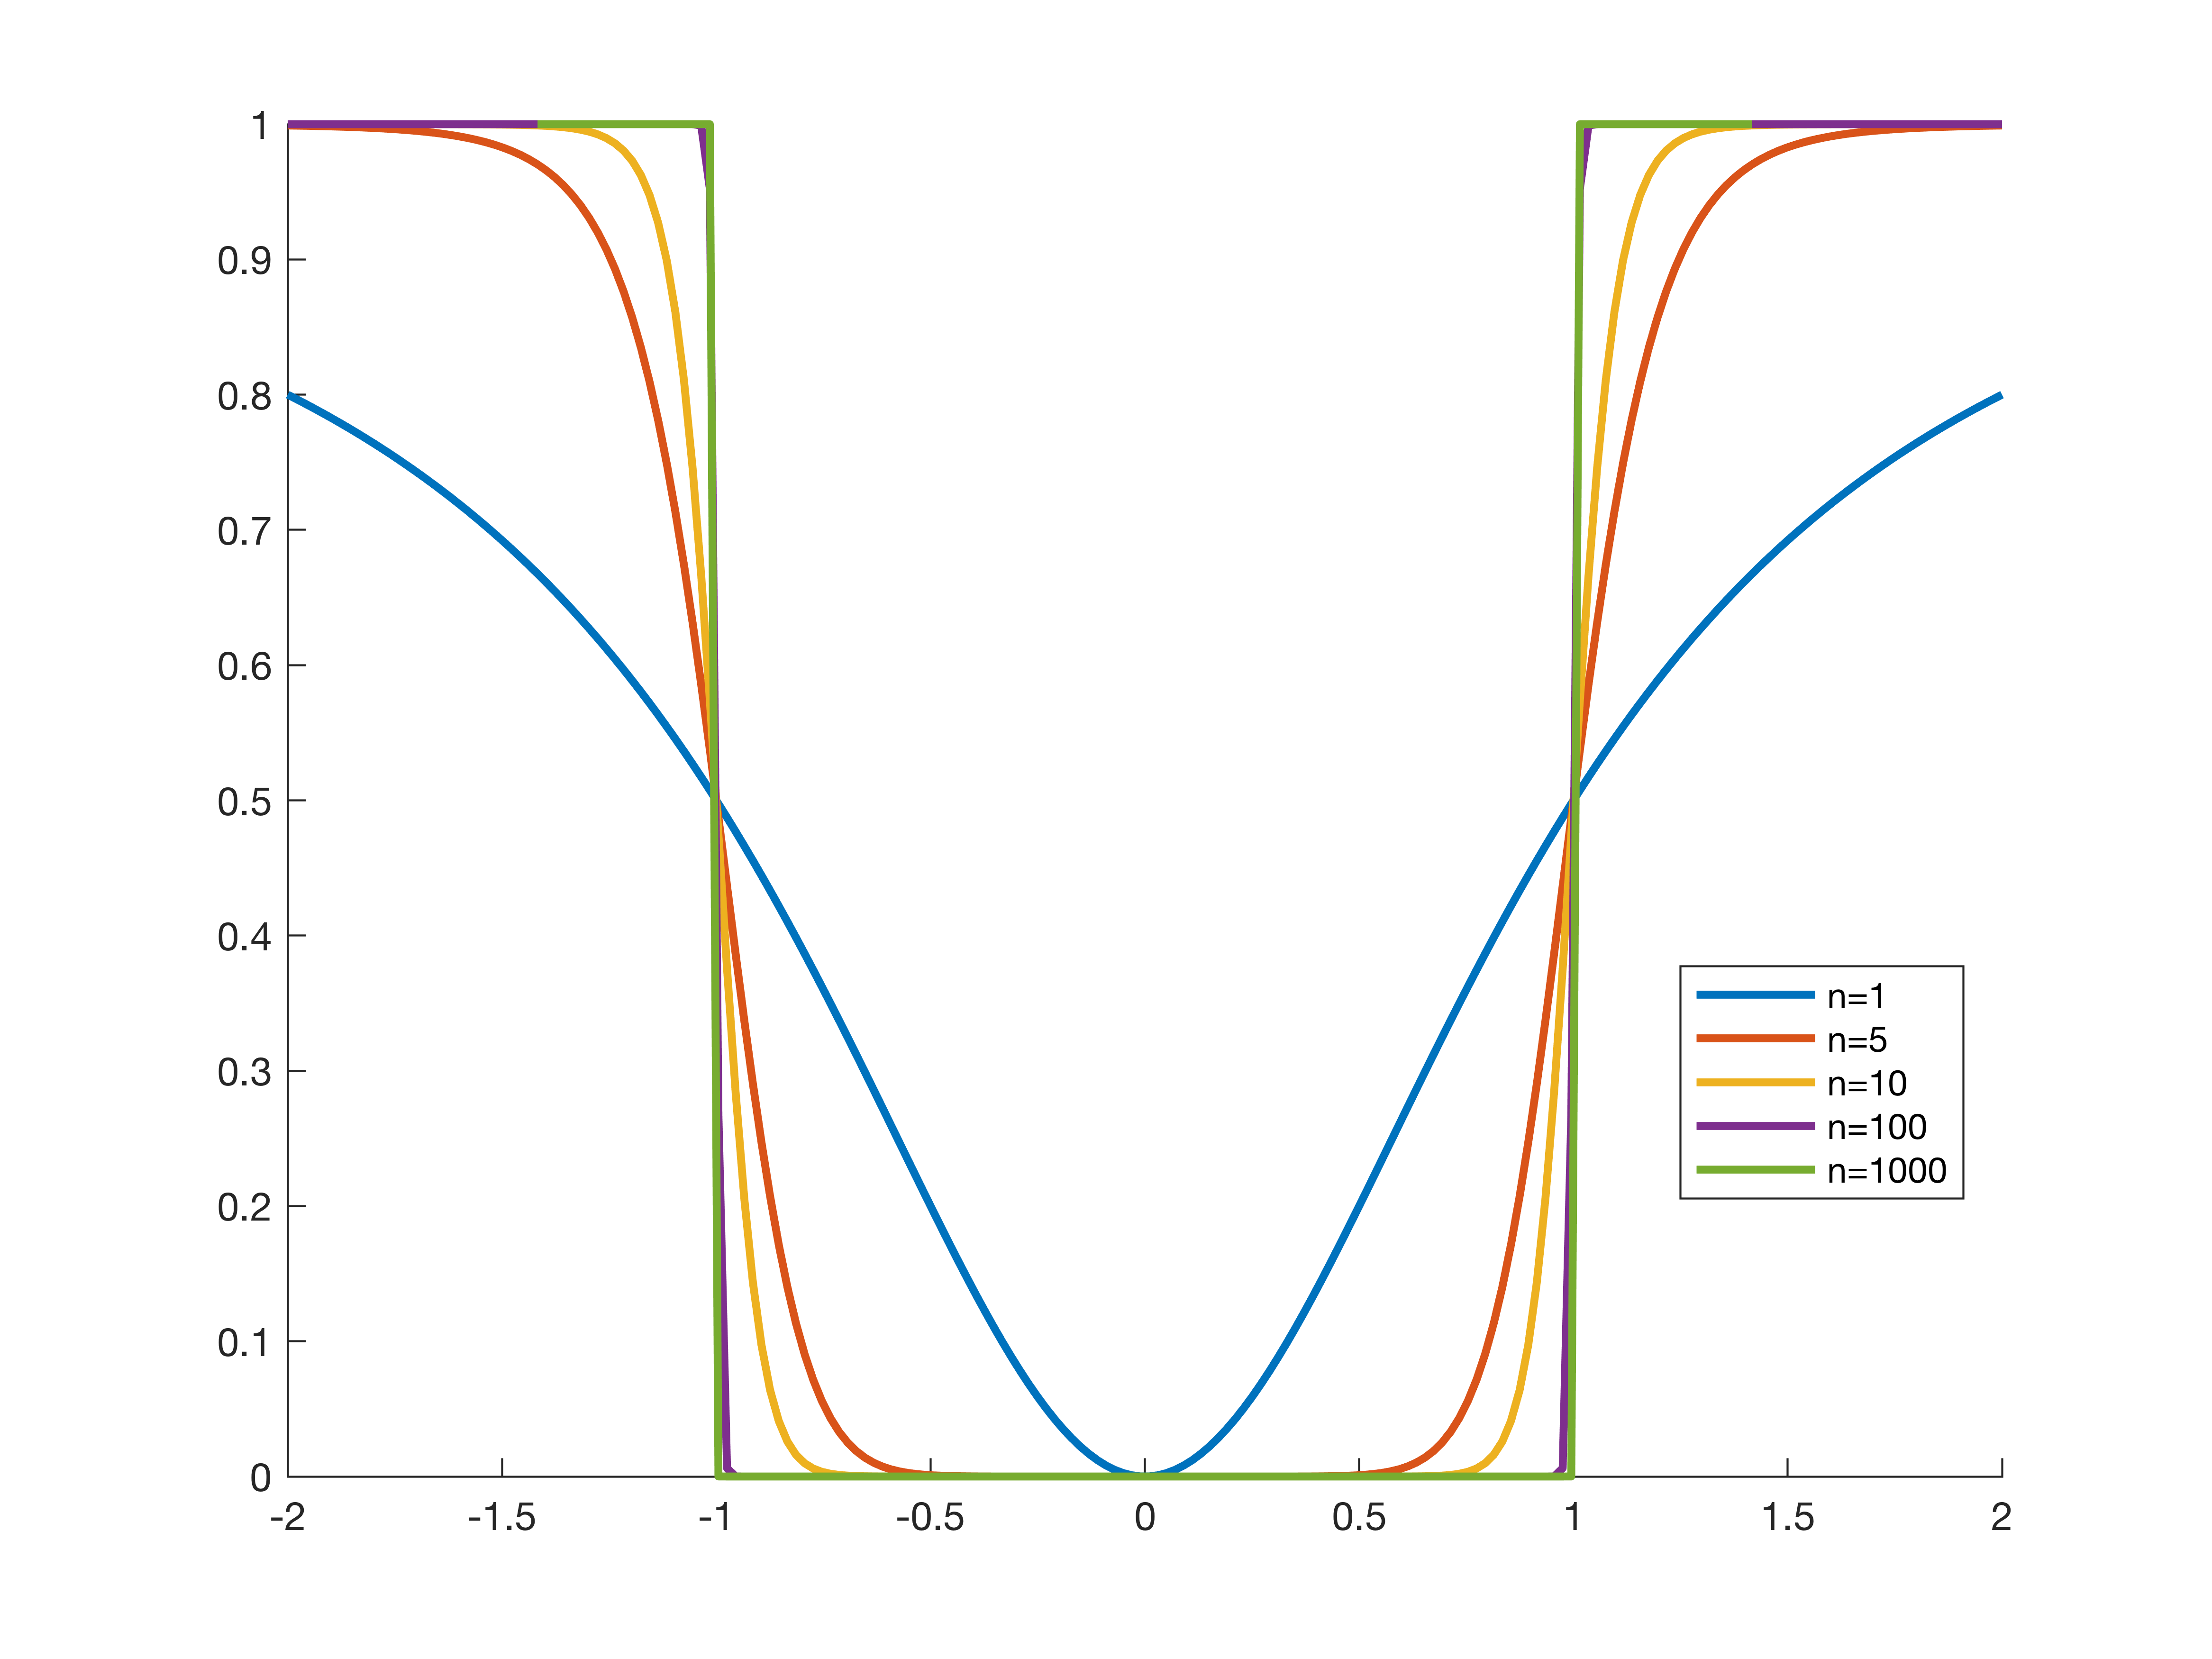
\includegraphics[width=.8\textwidth]{figure/fig1.png}
    %\includegraphics[width=2in]{XeTeX-2.jpg} 
    %\caption{An Numerical Example with $\alpha = 0.3, \beta = 0.98$}
    \end{figure}
\end{example}

\underline{Uniform Convegence} of $\{f_n\}$

Let $\{f_n\}$ be a sequence of functions that converges pointwise on a set $S$ to a limit function $f$, i.e., $\forall ~ x \in S$ and $\forall ~ \epsilon > 0$, $\exists ~ N \in \mathbb{N}$, where $N = N(x, \epsilon)$, s.t. 
\[
    \forall ~ n > N, |f_n(x) - f(x)| < \epsilon.
\]
\underline{Definition}: A sequence of functions $\{f_n\}$ is said to \underline{converge uniformly} to $f$ on a set $S$ if $\forall ~ \epsilon > 0$, $\exists ~ N(\epsilon) \in \mathbb{N}$, s.t. 
\[
    \forall ~ n > N, |f_n(x) - f(x)| < \epsilon, ~ \forall x \in S
\]

\underline{Geometry}

If $f_n$ is real-valued $\forall n \in \mathbb{N}$, then $| f_n(x) - f(x) | < \epsilon $ mean  
$$ f(x) - \epsilon  < f_n(x)  < f(x)  + \epsilon .$$
If this holds for all $n > N$ and for all $x \in S$, then $\{(x,y) \mid y = f_n(x), x \in S \}$, the entire graph, lies within the $2 \epsilon $ ``bound'' around $f$.

\begin{figure}[htbp] 
    \centering
    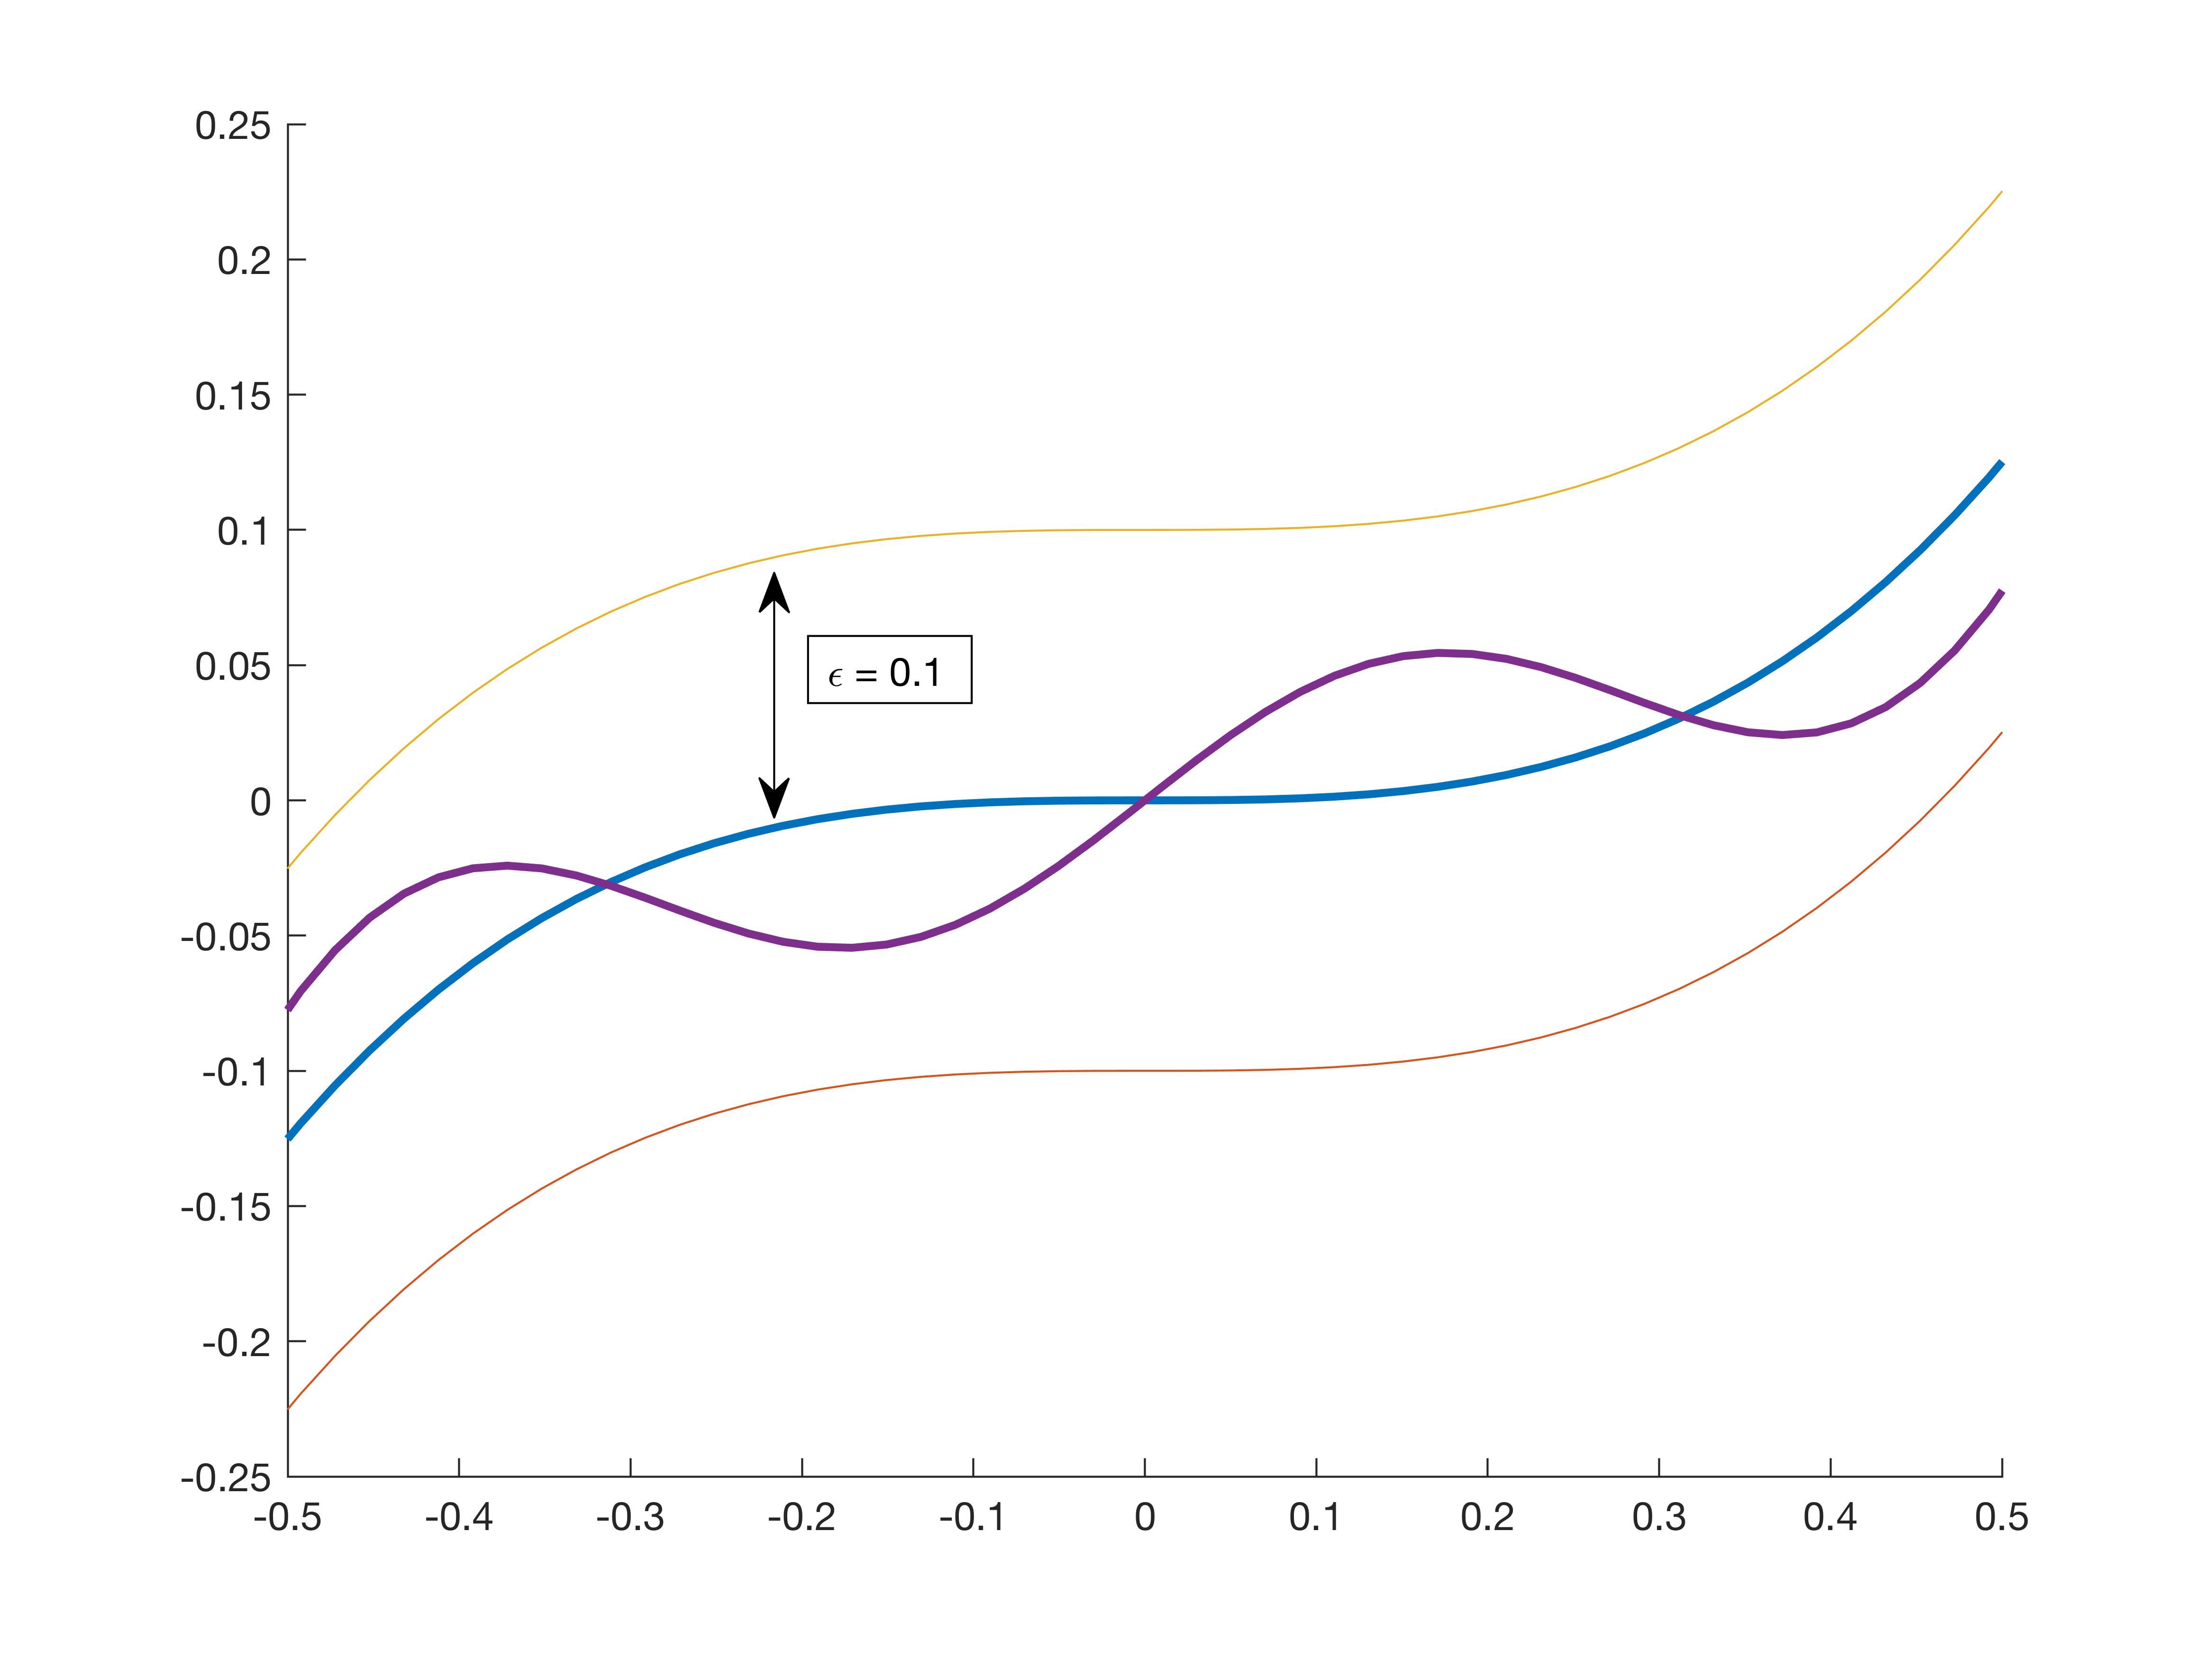
\includegraphics[width=.8\textwidth]{figure/fig2.png}
    %\includegraphics[width=2in]{XeTeX-2.jpg} 
    %\caption{An Numerical Example with $\alpha = 0.3, \beta = 0.98$}
\end{figure}

\underline{Uniform Bounds}
$\{f_n\}$ is \underline{uniformly bounded} on $S$ if $\exists M > 0$, constant, s.t. $|f_n(x)| \leq M , ~ \forall x \in S$ and $ \forall n$. The number $M$ is called a \underline{uniform bound} for $f_n$.

\underline{Theorem}(Apostol)

If $f_n \to f$ uniformly on $S$ and if each $f_n$ is bounded on $S$, then $f_n$ is uniformly bounded on $S$.

\underline{Theorem} (Uniform Convergence and Continuity, Apostol)

Let $f_n \to f$ uniformly on $S$. If each $f_n$ is continuous at a point $c \in S$, then the limit function $f$ is also continuous at $c$.

\underline{Theorem} (Cauchy Condition for Uniform Convergence)

Let $\{f_n\}$ be defined on $S$. Then there exists $f$ s.t. $f_n \to f$ uniformly on$S$ iff $\forall \epsilon >0, ~\exists~ N \in \mathbb{N}$ s.t. $\forall m,n > N$, \[
\underbrace{|f_m(x)- f_n(x)| }_{\text{Cauchy Condition}} < \epsilon, \quad \forall x \in S
\]

\begin{proof}
    ``\imp''

    Assume that $f_n \to f$ uniformly on $S$. Let $\epsilon >0$. Then $\exists N \in \mathbb{N}$ s.t. $n > N \Longrightarrow |f_n(x) - f(x)| < \frac{\epsilon}{2}, \forall x \in S$. Let $m >N$. Then $|f_m(x) - f(x)| < \frac{\epsilon}{2}$. Then 
    \[
    |f_m(x) - f_n(x)| = |f_m(x) - f(x) + f(x)- f_n(x)| \leq |f_m(x) - f(x)| + |f(x)- f_n(x)| < \frac{\epsilon}{2} + \frac{\epsilon}{2} = \epsilon
    \]

    ``$\Longleftarrow$''

    Suppose that the Cauchy condition is satisfied \imp $\forall x \in S, \{f_n(x)\}$ converges. 

    Let $f(x) = \lim_{n \to \infty} f_{n}(x) ~\forall~x \in S$.

    Let $\epsilon > 0$ and choose $N \in \mathbb{N}$ s.t. $\forall n > N$, \[
    |f_n(x) - f_{n+k}(x)| < \frac{\epsilon}{2}, \quad \forall k = 1,2,3 ..., \quad \forall x \in S.
    \]
    Then \[
    \lim_{k \to \infty} |f_n(x) - f_{n+k}(x)| = |f_n(x) - f(x)| \leq \frac{\epsilon}{2}
    \]
    \imp $\forall n > N$,
    \[
    |f_n(x) - f(x)| < \epsilon \quad \forall x \in S.
    \]
    \imp $f_n \to f$ uniformly on S.
\end{proof}








%$$##
\clearpage
\section*{References}
%\beginrefs
%\bibentry{CW87}{\sc D.~Coppersmith} and {\sc S.~Winograd}, 
%``Matrix multiplication via arithmetic progressions,''
%{\it Proceedings of the 19th ACM Symposium on Theory of %Computing},
%1987, pp.~1--6.
%\endrefs

% **** THIS ENDS THE EXAMPLES. DON'T DELETE THE FOLLOWING LINE:

\end{document}






















\section{First Order Linear Difference Equations}
\begin{equation}
    \underbrace{y_{t}}_{Endog.} = \lambda y_{t-1} + b \underbrace{x_t}_{Exog.} + a, \qquad a, b, \lambda = \text{ parameters, } \lambda \neq 1
\end{equation}
\underline{Note}:

$\lambda = 1$ unit root, non-stationary, random walk

\underline{Sargent 1979, CH.9}

\begin{equation}
    y_{y} - \lambda y_{t-1} = b x_{t} + a
\end{equation}
\begin{equation}
    (1- \lambda L)y_{t} = b x_{t} + a
\end{equation}
\begin{equation}
    y_{t} = \frac{1}{1 - \lambda L}(b x_{t}+a) + {c \lambda^{t}}
\end{equation}
where ${c \lambda^{t}}$ is the ``summation constant'', similar to the constant in indefinite integral. We can check that $$(1- \lambda L){c \lambda^{t}} = c \lambda^{t} - \lambda L (c \lambda^{t}) = c \lambda^{t} - \lambda c \lambda^{t-1} = 0$$

\underline{Note}
\begin{eqnarray}
    L(x_{t} \pm y_{t}) = x_{t-1} \pm y_{t-1}\\
    L(a x_{t}) = a L x_{t} =  a x_{t-1}\\
    y_t = (\frac{1}{1- \lambda L})b x_{t} + (\frac{1}{1- \lambda L}) a + c \lambda^t
\end{eqnarray}

\underline{Assuptions}

$|\lambda| < 1 \Longrightarrow La = a$.

Then
\begin{equation}
   ( \frac{1}{1- \lambda L})a = (\frac{1}{1- \lambda})a
\end{equation}
This is because
\begin{equation}
    ( \frac{1}{1- \lambda L})a = (\sum_{i=0}^{\infty} \lambda^{i}L^{i})a = \sum_{i=0}^{\infty} (\lambda^{i}L^{i}a) = \sum_{i=0}^{\infty} (\lambda^{i}a) = a \sum_{i=0}^{\infty} \lambda^{i} = a(\frac{1}{1- \lambda})
\end{equation}
Thus, 
\begin{equation}
\begin{aligned}
    y_t &= (\frac{1}{1- \lambda L})b x_{t} + (\frac{1}{1- \lambda L}) a + c \lambda^t\\
        &= b \sum_{i=0}^{\infty} \lambda^i x_{t-i} + \frac{a}{1- \lambda} + c \lambda^t
\end{aligned}
\end{equation}

\underline{Recall}

If $|\lambda|<1$, then $(\frac{1}{1- \lambda L}) x_{t} = \sum_{i=0}^{\infty} \lambda^i x_{t-i}$

If $|\lambda|>1$, then $(\frac{1}{1- \lambda L}) x_{t} = -\sum_{i=1}^{\infty} {(\frac{1}{\lambda})}^i x_{t+i}$

\underline{Note}: If $|\lambda| > 1$, then we would use forward-looking solution.

\begin{example} Cagan (1956)
\begin{equation}
    \begin{cases}
        m_t &= \ln M_{t}\\
        p_{t} &= \ln P_{t}\\
        p^e_{t+1} &= \ln P^{e}_{t+1}  
    \end{cases}
\end{equation}
\underline{Money Market}: Money demand
\begin{equation}
    \underbrace{m_t - p_t}_{\ln (\frac{M_t}{P_t})} = \alpha (\underbrace{p^e_{t+1} - p_{t}}_{\text{expeced inflation}}), \qquad \alpha <0
\end{equation}
this is a(n) simplification/approximation under hyperinflation:
\begin{equation}
    (\frac{M}{P})^{d} = \frac{M}{P}(i, y) = \frac{M}{P}(r + {\pi^{e}}, y) 
\end{equation}
When inflation is high, $r$ and $y$ can be treated as fixed.

\underline{Assumption}
$$y = \bar{y}, r = \bar{r}$$
\begin{equation}
    P^{e}_{t+1} = (1-\gamma) P_{t} + \gamma P_{t-1} \Longrightarrow \pi_{t+1}^{e} = \Gamma \pi_{t}, \quad \Gamma < 0
\end{equation}
which is an example of \underline{extrapolative} expectation.
\begin{equation}
    p_{t+1}^{e} = (1+ \Gamma)p_{t} - \Gamma p_{t-1}
\end{equation}
\begin{equation}
    m_{t} - p_{t} = \alpha \Gamma (p_{t}-p_{t-1})
\end{equation}
\begin{equation}
    \Longrightarrow p_{t} - \underbrace{(\frac{a \Gamma}{1 + a \Gamma})}_{\lambda} p_{t-1} = m_{t}
\end{equation}
\begin{equation}
    p_{t} - \lambda p_{t-1} = m_{t}
\end{equation}
\begin{equation}
    p_{t} = (\frac{1}{1 - \lambda L})m_{t} + c \lambda^{t}
\end{equation}
Since $|\lambda| = |\frac{\alpha \Gamma}{1+ \alpha \Gamma} | < 1$, \imp
\begin{equation}
    p_{t} = \sum_{i=0}^{\infty} \lambda^{i} m_{t-i} + c \lambda^{t} = \sum_{i=0}^{\infty} (\frac{\alpha \Gamma}{1+ \alpha \Gamma})^{i} m_{t-i} + c (\frac{\alpha \Gamma}{1+ \alpha \Gamma})^{t}
\end{equation}
\end{example}

\begin{example}
\underline{Perfect forsight}
    \begin{equation}
        p^{e}_{t+1} - p_{t} = p_{t+1} - p_{t}
    \end{equation}
    \begin{equation}
        \pi^{e}_{t+1} = \pi_{t+1}
    \end{equation}
    Then money demand is 
    \begin{equation}
        m_{t} - p_{t} = \alpha (p_{t+1} - p_{t})
    \end{equation}
    \begin{equation}
        \Longrightarrow p_{t+1} - \frac{\alpha-1}{\alpha}p_{t} = \frac{m_{t}}{\alpha}
    \end{equation}
    \begin{equation}
        \Longrightarrow (1 - \lambda L) p_{t+1} = \frac{m_{t}}{\alpha}
    \end{equation}
    Here, $|\lambda| = | \frac{\alpha-1}{\alpha}| > 1$. Hence use backward-looking solution:
    \begin{equation}
        \begin{aligned}
            p^{t+1} 
            &= - \frac{1}{\alpha} \left ( \frac{1}{1 - \lambda L} \right ) m_{t} + c \lambda^{t}\\
            &= - \frac{1}{\alpha} \sum_{i=1}^{\infty} \left ( \frac{1}{\lambda} \right )^i m_{t+i} + c \lambda^{t}\\
            &= - \frac{1}{\alpha} \sum_{i=1}^{\infty} \left ( \frac{1}{(\frac{\alpha-1}{\alpha})} \right )^i m_{t+i} + c (\frac{\alpha-1}{\alpha})^{t}\\
            &= \frac{1- \alpha}{\alpha^2} \sum_{i=1}^{\infty} \left ( \frac{\alpha}{\alpha-1} \right )^{i+1} m_{t+i} + c (\frac{\alpha-1}{\alpha})^{t}\\
            p_{t} &= \frac{1- \alpha}{\alpha^2} \sum_{i=1}^{\infty} \left ( \frac{\alpha}{\alpha-1} \right )^{i+1} m_{t+i-1} + c (\frac{\alpha-1}{\alpha})^{t-1}
        \end{aligned}
    \end{equation}
\end{example}

\section{Dynamic Discrete Time Infinite Horizon Model (Ramsey)}
\begin{equation}
    \max \quad \sum_{t=1}^{\infty} \beta^{t} u(c_{t}), \qquad 1 > \beta > 0
\end{equation}
\begin{equation}
    \text{s.t.} \quad c_t + B_{t} = (1+ \rho_{t-1}) B_{t-1} + y_{t}
\end{equation}
\begin{equation}
    \mathcal{L} = \sum_{t=1}^{\infty} \beta^{t} u(c_{t}) -  \sum_{t=1}^{\infty} \lambda_{t} [(1+ \rho_{t-1}) B_{t-1} + y_{t} - c_t - B_{t}]
\end{equation}
\underline{Choice}: $\{c_{t}, B_{t}\}_{t=1}^{\infty}$

\underline{FONC}:
\begin{eqnarray}
    &[c_{t}]& \qquad \beta^{t} u'(c_{t}) - \lambda_{t} = 0\\
    &[B_t]& \qquad -\lambda_{t} + \lambda_{t+1}(1+\rho_{t}) = a
\end{eqnarray}
\imp
\begin{equation}
    1 + \rho_{t} = \frac{u'(c_{t})}{\beta u'(c_{t+1})}
\end{equation}
which says ``objective rate of substitution'' = ``subjective rate of substitution''.

\underline{Assumption}: $\rho_{t} = \rho, ~ \forall t$ 
\begin{equation}
    (1 - (1+ \rho)L)B_{t} = y_{t} - c_{t}
\end{equation}
\begin{eqnarray}
    B_{t} 
    &=& \frac{1}{1 - (1+ \rho)L}(y_{t} - c_{t})\\
    &=& - \sum_{s=1}^{\infty} (\frac{1}{1+\rho})^{s}(y_{t+s}-c_{t+s}) + d (1 + \rho)^{t}\\
    &=& - \sum_{s=1}^{\infty} (\frac{1}{1+\rho})^{s}(y_{t+s}-c_{t+s}) \qquad (d = 0 \text{ because of NPGC})\\
    \sum_{s=1}^{\infty} (\frac{1}{1+\rho})^{s} c_{t+s} &=& B_{t} + \sum_{s=1}^{\infty} (\frac{1}{1+\rho})^{s} y_{t+s} 
\end{eqnarray}
which is the life-time budget constaint.

\underline{NPGC}:
\begin{equation}
    \lim_{t \to \infty} d(1+\rho)^{t} = 0 \Longrightarrow d = 0
\end{equation}

\underline{Assumption} $y_{t} = y, ~u(c) = \ln(c)$ \imp
\begin{equation}
    1 + \rho = \frac{1}{\beta }\frac{c_{t+1}}{c_{t} } \iff (1 + \rho)\beta c_{t} = c_{t+1}
\end{equation}
\begin{eqnarray}
    c_{t+1} &=& (1 + \rho)\beta c_{t}\\
    c_{t+2} &=& ((1 + \rho)\beta)^2 c_{t}\\
    c_{t+3} &=& ((1 + \rho)\beta)^3 c_{t}\\
    &\vdots&\\
    c_{t+s} &=& ((1 + \rho)\beta)^s c_{t}
\end{eqnarray}
\imp
\begin{equation}
    B_{t} + \sum_{s=1}^{\infty} (\frac{1}{1+\rho})^{s}y = 
     \sum_{s=1}^{\infty} (\frac{1}{1+\rho})^{s} (1 + \rho)^{s}\beta^{s} c_{t}
\end{equation}
\begin{equation}
    B_{t} + y \sum_{s=1}^{\infty} (\frac{1}{1+\rho})^{s} = 
     c_{t} \sum_{s=1}^{\infty} \cancel{(\frac{1}{1+\rho})^{s} (1 + \rho)^{s}}\beta^{s} 
\end{equation}
\begin{equation}
    B_{t} + \frac{1}{\rho}y = \frac{\beta}{1-\beta} c_{t}
\end{equation}
%Assume $\beta = \rho$, then we have
\begin{equation}
    c_t = \frac{1- \beta}{\beta \rho}(y + \rho B_{t})
\end{equation}

\section{Expectations}
How to get information about expectation?
\begin{enumerate}
    \item Survey
    \item Observe behaviour
    \item Assume some mechanism
    \begin{enumerate}
        \item Static expectation $p^{e}_{t+1} = p_{t}$\\
        Example: The cobweb model
        \item Extrapolative expectations\\
        Example:
        \begin{equation}
            p^{e}_{t+1} = \Gamma p_{t} + (1- \Gamma)p_{t-1} = \Gamma (p_{t} - p_{t-1}) + p_{t-1}
        \end{equation}
        Example:
        \begin{equation}
        \begin{aligned}
            C_{t+1} &= \alpha + \beta y^{e}_{t+1}\\
            &= \alpha + \beta \Gamma y_{t} + \beta (1- \Gamma) y_{t-1} + \epsilon_{t}
        \end{aligned}
        \end{equation}
        \item Adaptive expectations
    \end{enumerate}
\end{enumerate}

\underline{Adaptive Expectations}
\begin{equation}
    p^{e}_{t+1} = p^{e}_{t} + \theta (\underbrace{p_{t} - p^{e}_{t}}_{\text{forecast error}}), \qquad 0 < \theta < 1
\end{equation}
\begin{equation}
    p^{e}_{t+1} = \theta \sum_{s=0}^{\infty}(1- \theta)^{s} p_{t-s} + c (1 - \theta)^{t}
\end{equation}

\underline{Rational Expectations}
\begin{itemize}
    \item [1)] $P^{e}_{t+1} = \E [P_{t+1} \mid \Omega_{t}]$
    \item [2)] $P^{e}_{t+1} - P_{t+1} = \epsilon_{t+1}$, where $\E (\epsilon_{t+1}) = 0$, $\text{cov}(\epsilon_{t}, \epsilon_{t \pm 1})$.
\end{itemize}
\underline{Perfect Forsight} is an extreme case of RE  where $\epsilon_{t+1} = 0 ~ \forall t$.

\section{Stochastic Difference Equation}
\begin{equation}
    y_{t} = a \underbrace{\E [y_{t+1} | I_{t}]}_{\E_{t} y_{t+1}} + c x_{t}
\end{equation}
\begin{example}
    \begin{equation}
        p_{t} = (\frac{\alpha}{1+ \alpha}) \E [p_{t+1}| I_{t}]+     (\frac{1}{1+ \alpha})m_{t}
    \end{equation}
\end{example}

\underline{Law of Iterated Expectations}
\begin{equation}
    \E \lsb \E \lsb X | I_{t+1} \rsb | I_t \rsb = \E \lsb X| I_{t} \rsb
\end{equation}

\begin{eqnarray}
    y_{t} &=& a \E_{t}y_{t+1} + c x_{t}\\
    y_{t+1} &=& a \E_{t+1}y_{t+2} + c x_{t+1}\\
    \E_{t} y_{t+1} &=& a \E_{t} \E_{t+1}y_{t+2} + c \E_{t} x_{t+1} = a \E_{t} y_{t+2} + c \E_{t} x_{t+1} \\
    \Longrightarrow 
    y_{t} &=& a^{2} \E_{t} y_{t+2} + a c \E_{t} x_{t+1} + c x_{t}\\
    y_{t+2} &=& a \E_{t+2}y_{t+3} + c x_{t+2}\\
    \Longrightarrow 
    \E_{t} y_{t+2} &=& a \E_{t}y_{t+3} + c \E_{t} x_{t+2}\\
    \Longrightarrow 
    y_{t} &=& a^{3} \E_{t} y_{t+3} + a^2 c \E_{t} x_{t+2} + a c \E_{t} x_{t+1} + c x_{t}\\
    &\vdots& \notag\\
    y_{t} &=& c \sum_{i=0}^{T} a^{i}\E_{t}x_{t+i} + a^{T+1} \E_{t} y_{t+T+1}
\end{eqnarray}
Let $T \to \infty$ and assume that \begin{equation}
    \lim_{T \to \infty} [a^{T+1} \E_{t}y_{t+T+1}] = 0
\end{equation}
i.e. we are ruling out  bubble solution.

Then we get the fundamental solution:
\begin{equation}
    y_{t} = c \sum_{i=0}^{\infty} a^{i} \E_{t} x_{t+i}
\end{equation}

\section{Stochastic Dynamic Discrete Time Infinite Horizon Model}
\begin{equation}
    \max \quad \E \lsb \sum_{t=1}^{\infty} \beta^{t} u(c_{t})  \rsb 
\end{equation}
\begin{equation}
    \text{s.t.} \quad c_t + B_{t} = (1+ \rho_{t-1}) B_{t-1} + y_{t}
\end{equation}
\underline{Random Lagrangian Method} (Kushner (1965))

\underline{FONC}
\begin{eqnarray}
    \E_{t} [ \beta^{t} u'(c_{t}) - \lambda_{t}] = 0\\
    \E_{t} [ - \lambda_{t} + \lambda_{t+1} (1+ \rho_{t})] = 0
\end{eqnarray}

\underline{Note}: At time t, variables dated $t$ and earlier are known and hence they are not R.V.'s (random variables), i.e.
\begin{equation}
    \E_{t} x_{t} = \E [x_{t} | I_{t} ] = x_{t}
\end{equation}
\imp
\begin{eqnarray}
    \beta^{t} u'(c_{t}) - \lambda_{t} = 0\\
    -\lambda_{t} + (1- \rho_{t}) \E_{t} \lambda_{t+1} = 0
\end{eqnarray}
\imp    
\begin{equation}
    u'(c_{t}) = (1- \rho_{t}) \beta \E_{t} u'(c_{t+1})
\end{equation}
\begin{equation}
    \E_{t} u'(c_{t+1}) = \frac{1}{(1- \rho_{t}) \beta} u'(c_{t})
\end{equation}
\begin{equation}
    u'(c_{t+1}) = \frac{1}{(1- \rho_{t}) \beta} u'(c_{t}) + \epsilon_{t+1}
\end{equation}
with $\E_{t} \epsilon_{t+1} = 0$. Hence it's almost an AR(1) process.

\underline{Claim}: If $\E_t (x_{t+1}) = x_{t}$, then $x_{t+1} = x_{t} + \epsilon_{t+1}$, $E_{t} \epsilon_{t+1} = 0$.

\underline{Comment}: This is also a regression equation/model that can be used for estimation, taken to data for test directly. If $u(c) = \ln c$, then \begin{equation}
    \frac{1}{c_{t+1}} = \frac{1}{(1- \rho_{t}) \beta}  \frac{1}{c_{t}} + \epsilon_{t+1}
\end{equation}
which is a regression equation with time-varying coefficient (Kalman). (F. Mishikin 1986, NBER-U.C. Press)

\underline{Assumption}: $\rho_{t} = \rho$ and $\beta = \frac{1}{1+ \rho}$

Then 
\begin{equation}
    u'(c_{t+1}) = u'(c_{t}) + \epsilon_{t+1}
\end{equation}
MU of consumption is a random walk.

With quadratic utility function, $\text{MU} = \alpha - \beta c$, Hall (1978) showed that
\begin{equation}
    c_{t+1} = c_{t} + \epsilon_{t+1}.
\end{equation}


